\section{Collection of dataset}
This chapter will go through how a dataset was collected containing only some specific beat boxing sounds.
For collection of the dataset containing beat boxing, only three type of different beat boxing sounds there was made use of a recorder, a microphone, a headset, some boards (to limit the noise from surroundings as much as possible) and a computer to take notes of when the different people did record their beat boxing, The setup of the place where the record took place and be seen on figure \ref{data-collection-pic}. For choosing the people to help us make the beatboxing random convenience method was used. 
\begin{figure}[h]
	\begin{center}
		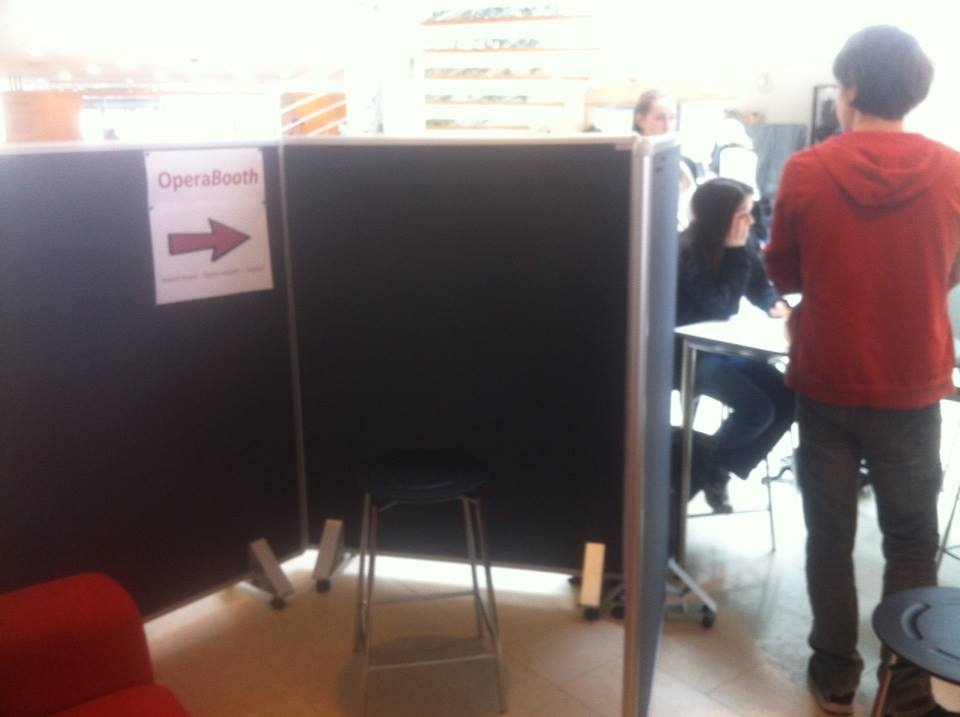
\includegraphics[height=5cm]{fig/dataset_collection.JPG}
		\caption{ place where the beatboxer participant was place during the recording of the data set, taken with a phone camera}
		\label{data-collection-pic}
	\end{center}
\end{figure}
When the participants sat in the stall they was asked to practice a few different beat boxing sounds, when they had learned one they would be recorded making that  sound this was repeated with three sounds, a kick drum beat boxing sound, a snare drum beat boxing sound and a hi-hat drum beat boxing sound. After they had made the three sounds they were also asked to improvise a short mix of the three beat boxing sounds that they had learned.
